\section{Ανάπτυξη Αθροιστών υπολοίπου $2^n-1$ }

Σε αυτό το κεφάλαιο θα αναπτυχθούν συνολικά δώδεκα αθροιστές υπολοίπου $2^n-1$
ακολουθώντας την αρχιτεκτονική που παρουσιάστηκε στο προηγούμενο κεφάλαιο 
με τα ελάχιστα επίπεδα. Ανάλογα με το είδος της παραγοντοποίησης που τους εφαρμόζεται 
οι αθροιστές ομαδοποιούνται σε τρεις ομάδες, Prefix, Ling και Jackson,
και σε κάθε ομάδα θα αναπτυχθεί ένας 8-bit, ένας 16-bit, ένας 32-bit και ένας 64-bit 
αθροιστής. Για κάθε ομάδα θα αναλύεται και σχηματικά ο 8-bit αθροιστής λόγω του 
ευδιάκριτου σχήματος που τον περιγράφει, ενώ για τους υπόλοιπους θα δοθεί η
συναρτησιακή λογική πλήρως σε άλγεβρα Μπουλ.




\subsection{Βασική δομή}
Στην εικόνα \ref{2^8-1_Tree_2x4} παρουσιάζεται προσεγγιστικά η δομή των αθροιστών υπολοίπου $2^8-1$ 
που θα χρησιμοποιηθεί παρακάτω. Ενώ η δομή είναι κοινή και για τα τρία είδη αθροιστών το κάθε σχήμα 
αντιπροσωπεί διαφορετική λογική συνάρτηση. Επίσης στο δέντρο αυτό ακολουθείται η καταστευέι μόνο 
των σημάτων που οδηγόυν τον τελευταίο πολυπλέκτη, δηλαδή στην περίπτωση του Prefix το σήμα G, στου Ling
το σήμα H και στο Jackson το R.
\begin{figure}[H]
\centering
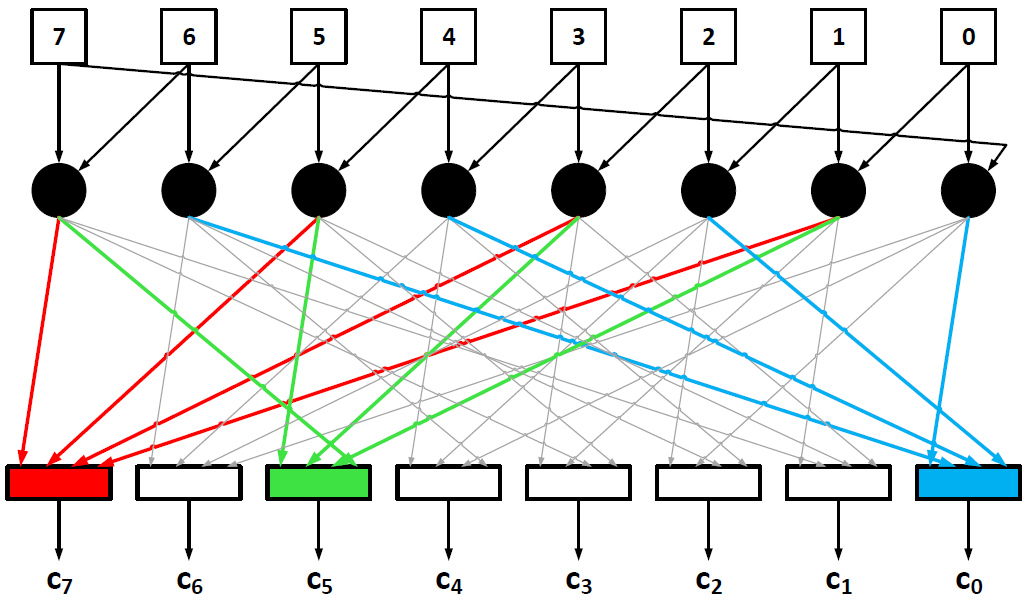
\includegraphics[width=\textwidth]{J8_Color.png}
\caption{Jackson 8-bit $2^n-1$ Adder}
\label{2^8-1_Tree_2x4}
\end{figure}







\subsection{Prefix $2^n-1$}
%\subsubsection{$2^8-1$}
%\subsubsection{$2^{16}-1$}
%\subsubsection{$2^{32}-1$}
%\subsubsection{$2^{64}-1$}


%---------------------------------------------------
\subsection{Ling $2^n-1$}
%---------------------------------------------------



%\subsubsection{$2^8-1$}
%%---------------------------------------------------
%\subsubsection{$2^{16}-1$}
%\subsubsection{$2^{32}-1$}
%\subsubsection{$2^{64}-1$}






%---------------------------------------------------
\subsection{Jackson $2^n-1$}
%---------------------------------------------------
Στην ενότητα \ref{section:jackson} έγινε μια αναφορά σε σχεδιαστικούς κανόνες όσο αφορά τους 
αθροιστές Jackson. Για την ανάπτυξη ενός Jacson αθροιστή υπάρχει ένα μεγάλο πλήθος πιθανών υλοποιήσεων,
όχι μόνο στην επιλογή του προθεματικού δέντρου και το πλήθος των όρων της παραγοντοποίησης ( Radix-2, 
Radix-3, Radix-4 ... ), κάτι που αφορά και τους αθροιστές Prefix και Ling, αλλά 
και στην επιλογή της συνάρτησης παραγοντοποίησης σε κάθε επίπεδο.
\\\\
\textcolor{red}{[Γράψε όλους τους συνδυασμούς για έναν 8-bit ή 16-bit αθροιστή σε συντομία
π.χ. για 8 = 2x2x2, 2x4, 4x2 , και σε κάθε ένα τις πιθανές Burgess Συναρτήσεις]}






\subsubsection{$2^8-1$}
%---------------------------------------------------

% Figure
%
%--------------------------------------------






Επίπεδο 1:\\
\begin{equation}
\begin{split}
p_i &= a_i + b_i\\
g_i &= a_i * b_i\\
x_i &= a_i \oplus b_i
\end{split}
\end{equation}
\\
Επίπεδο 2:\\
\begin{equation}
\begin{split}
R^1_{i:i-1} &= g_i + g_{i-1}\\
Q^1_{i:i-1} &= p_i * p_{i-1}\\
\end{split}
\end{equation}
\\
Επίπεδο 3:\\
\begin{equation}
\begin{split}
R^3_{i:i-7} =& R^1_{i:i-1} + R^1_{i-2:i-3} + Q^1_{i-3:i-4} R^1_{i-4:i-5} \\
            +& Q^1_{i-3:i-4} Q^1_{i-5:i-6} R^1_{i-6:i-7} 
\end{split}
\end{equation}
\\
Group Generate:\\
\begin{equation}
G_{i:i-7} = D_{i:i-2} R^3_{i:i-7}
\end{equation}
Όπου : 
\begin{equation}
\begin{split}
D_{i:i-2} &= G_{i:i-1} + P_{i:i-2}\\
D_{i:i-2} &= g_i + p_ig_{i-1} + p_ip_{i-1}p_{i-2}
\end{split}
\end{equation}
\\
Επίπεδο 5 - Sum computation:\\
\begin{equation}
% sum_i = !R^3_{i-1:i-8} * (a_i \oplus b_i) + R^3_{i-1:i-8} * (a_i \oplus b_i \oplus D_{i-1:i-3})
sum_i = R^3_{i-1:i-8} ? (x_i \oplus D_{i-1:i-3}) : x_i
\end{equation}






Για παράδειγμα:\\
\rule{\linewidth}{0.5mm}
\begin{equation*}
\begin{split}
p_7 =& a_7 + b_7\\
g_7 =& a_7 * b_7\\
R^1_{7:6} =& g_7 + g_{6}\\
Q^1_{7:6} =& p_7 * p_{6}\\
R^3_{7:0} =& R^1_{7:6} + R^1_{5:4} + Q^1_{4:3} R^1_{3:2} + Q^1_{4:3} Q^1_{2:1} R^1_{1:0}\\
D_{7:5} =& g_7 + p_7g_{6} + p_7p_{6}p_{5}\\
sum_7 =& !R^3_{6:7} * (a_7 \oplus b_7) + R^3_{6:7} * (a_7 \oplus b_7 \oplus D_{6:4})
\end{split}
\end{equation*}
\rule{\linewidth}{0.5mm}











\subsubsection{Λογική περιγραφή των $2^{16}-1$,$2^{32}-1$ και $2^{64}-1$,}
\rule{\linewidth}{0.5mm}
\begin{equation*}
\begin{split}
p_7 =& a_7 + b_7\\
g_7 =& a_7 * b_7\\
R^1_{7:6} =& g_7 + g_{6}\\
Q^1_{7:6} =& p_7 * p_{6}\\
R^3_{7:0} =& R^1_{7:6} + R^1_{5:4} + Q^1_{4:3} R^1_{3:2} + Q^1_{4:3} Q^1_{2:1} R^1_{1:0}\\
D_{7:5} =& g_7 + p_7g_{6} + p_7p_{6}p_{5}\\
sum_7 =& !R^3_{6:7} * (a_7 \oplus b_7) + R^3_{6:7} * (a_7 \oplus b_7 \oplus D_{6:4})
\end{split}
\end{equation*}
\rule{\linewidth}{0.5mm}























%\subsubsection{$2^{16}-1$}
%%---------------------------------------------------
%Για παράδειγμα:\\
%\rule{\linewidth}{0.5mm}
%\begin{equation*}
%\begin{split}
%R^1_{15:12} =& g_{15} + g_{14} + p_{14}g_{13} + p_{14}p_{13}g_{12}\\
%Q^3_{15:12} =& p_{15} * p_{14} * p_{13} * p_{12}\\
%R^5_{15:0} =& R^1_{15:12} + R^1_{11:8} + Q^3_{10:7} R^1_{7:4} + Q^3_{10:7} Q^3_{6:3} R^1_{3:0}\\
%D_{15:11} =& p_{15}R^1_{15:12} + p_{11}Q^3_{15:12} \\
%sum_15 =& !R^5_{14:15} * (a_15 \oplus b_15) + R^5_{14:15} * (a_15 \oplus b_15 \oplus D_{14:10})
%\end{split}
%\end{equation*}
%\rule{\linewidth}{0.5mm}




%\subsubsection{$2^{32}-1$}
%%---------------------------------------------------
%
%
%
%
%
%\subsubsection{$2^{64}-1$}
%%---------------------------------------------------
%Για παράδειγμα:\\
%\rule{\linewidth}{0.5mm}
%\begin{equation*}
%\begin{split}
%R^1_{63:60} =& g_{63} + g_{62} + p_{62}g_{61} + p_{62}p_{61}g_{60}\\
%Q^3_{63:60} =& p_{63} * p_{62} * p_{61} * p_{60}\\
%R^5_{63:48} =& R^1_{63:60} + R^1_{59:56} + Q^3_{58:55} R^1_{55:52} + Q^3_{58:55} Q^3_{54:51} R^1_{51:48}\\
%Q^{11}_{63:48} =& Q^3_{63:60} Q^3_{59:56} Q^3_{55:52} ( R^1_{52:49} + Q^3_{51:48})\\
%R^{11}_{63:0} =& R^5_{63:48} + R^5_{47:32} + Q^{11}_{42:27} R^5_{31:16} + Q^{11}_{42:27} Q^{11}_{26:11} R^5_{15:0}\\
%D_{63:61} =& g_{63} + p_{63}g_{62} + p_{63}p_{62}p_{61}\\
%D_{63:59} =& D_{63:61} [R^1_{63:60} + Q^3_{62:59}]\\
%D_{63:43} =& D_{63:59} [R^5_{63:48} + Q^{11}_{58:43}]\\
%sum_63 =& !R^5_{62:63} * (a_63 \oplus b_63) + R^5_{62:63} * (a_63 \oplus b_63 \oplus D_{62:42})\\
%\end{split}
%\end{equation*}
%\rule{\linewidth}{0.5mm}

